%%%%%%%%%%%%%%%%%%%%%%%%%%%%%%%%%%%%%%%%%%%%%%%%%%%%%%%%%%%%%%%%%%%%%%%%%%%%%
%	e-Yantra, IIT-Bombay

%	Document Author: Chinmay Patil
%	Date: 11-July,2016
%	Last Edited by: Chinmay
%   Date Last updated: 11-06-2016 

%%%%%%%%%%%%%%%%%%%%%%%%%%%%%%%%%%%%%%%%%%%%%%%%%%%%%%%%%%%%%%%%%%%%%%%%%%%%%


\documentclass[11pt,a4paper]{article}
\usepackage{graphicx}
\usepackage{listings}
\usepackage{graphics}
\usepackage{wrapfig}
\usepackage[T1]{fontenc}
\usepackage[margin=1.2in]{geometry}
\usepackage{tcolorbox}
\usepackage{hyperref}
\usepackage{dingbat}
\usepackage{float}
\usepackage{tocloft}


\begin{document}
\begin{titlepage}
\title{Recovering the Firmware}
\author{e-Yantra Team}
\date{\today}
\maketitle
\end{titlepage}
 \tableofcontents
 
 
 \newpage
	\section{Prerequisites}
	\begin{itemize}
	\item You need to have an account on www.cypress.com inorder to download wiced sdk.
	\item A windows running machine.
	\item Knowledge about C programming.
	\item Read the Programming Wiced with Wiced SDK document in this repo.
	\end{itemize}
	
	\section{Hardware Requirement}
	\begin{itemize}
	\item Wiced Sense Tag
	\item A local system (Laptop or PC with bluetooth 4.0 or above)
	\item Micro Usb Cable
	\end{itemize}
	
	\section{Software Requirement}
	\begin{itemize}
	\item Wiced Sense SDK
	\end{itemize}
	
	
\newpage
\section{Recovery Procedure}
	\begin{enumerate}
	  \item Remove the CR2032 battery by opening the cover on the back of the wiced sense.
	  \begin{figure}[h]
        \centering
    	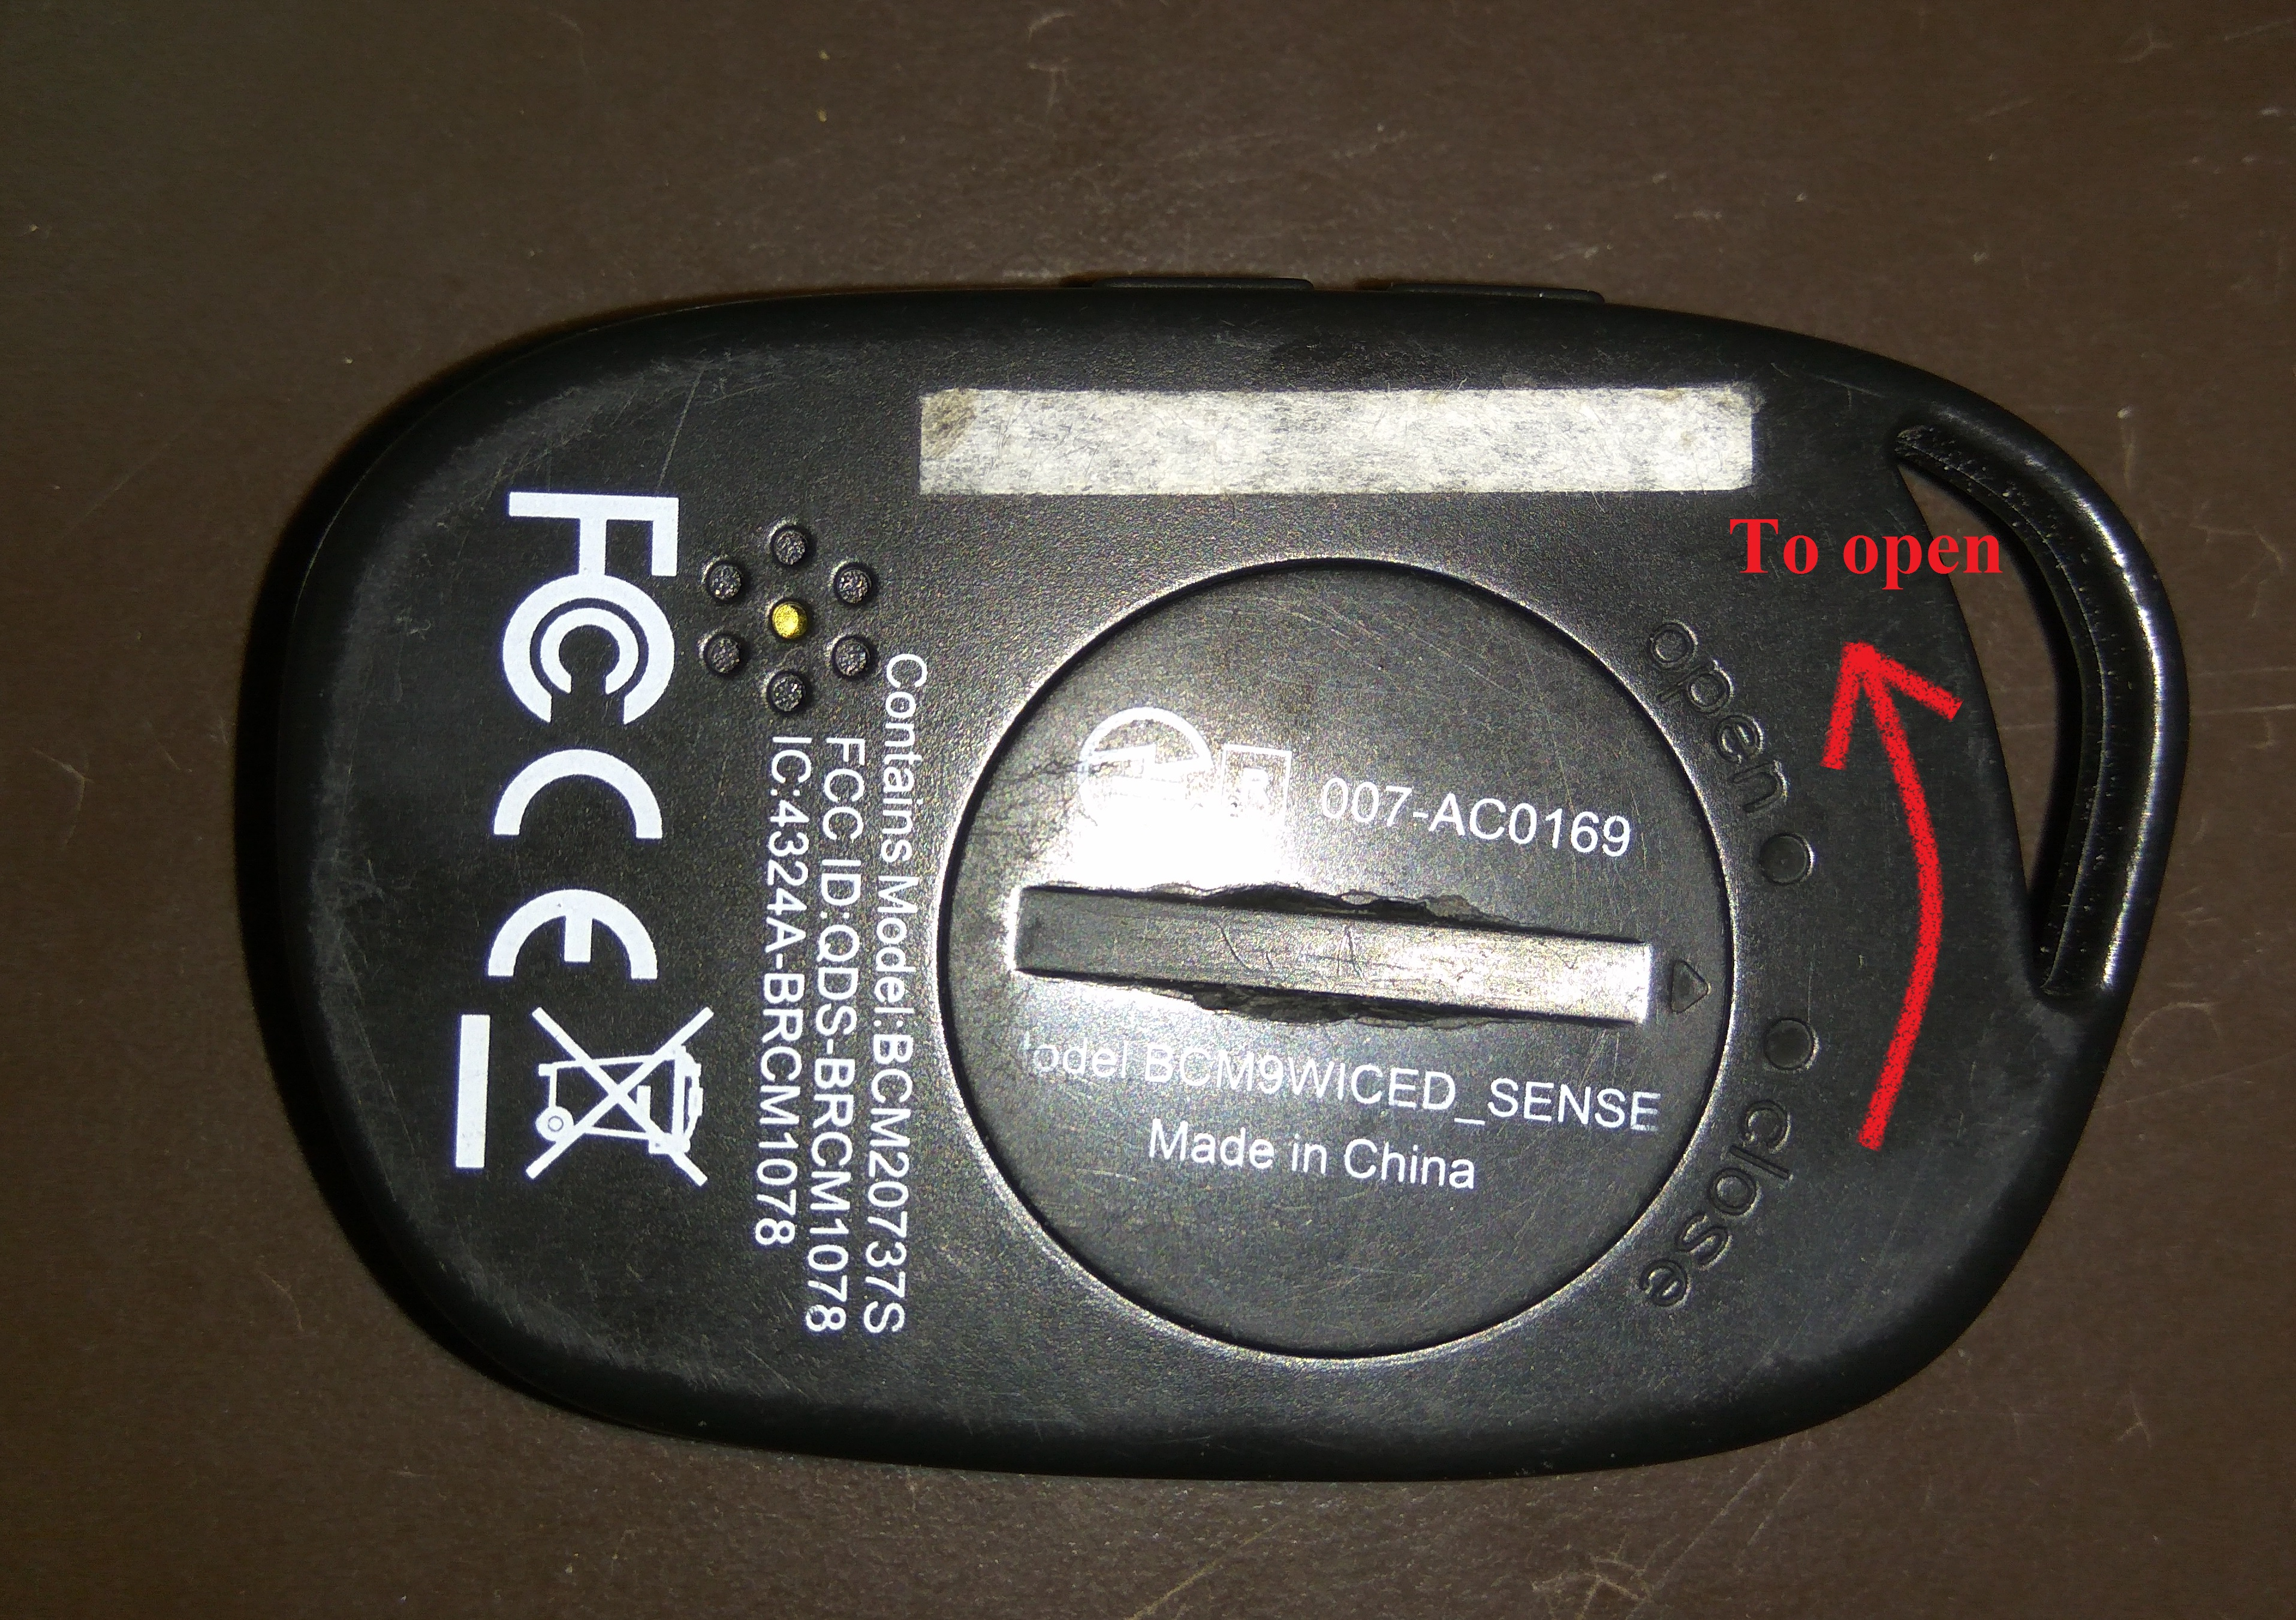
\includegraphics[scale=0.05]{1.jpg}
	    \end{figure}
	     \begin{figure}[h]
        \centering
    	\includegraphics[scale=0.05]{2.jpg}
	    \end{figure}
	  \item Open the Wiced sense device. The top housing do not have any screws, it is attached by locking mechanism. Open it with a screw driver by pushing it from the space where we place the battery.
	  
	   \begin{figure}[h]
        \centering
    	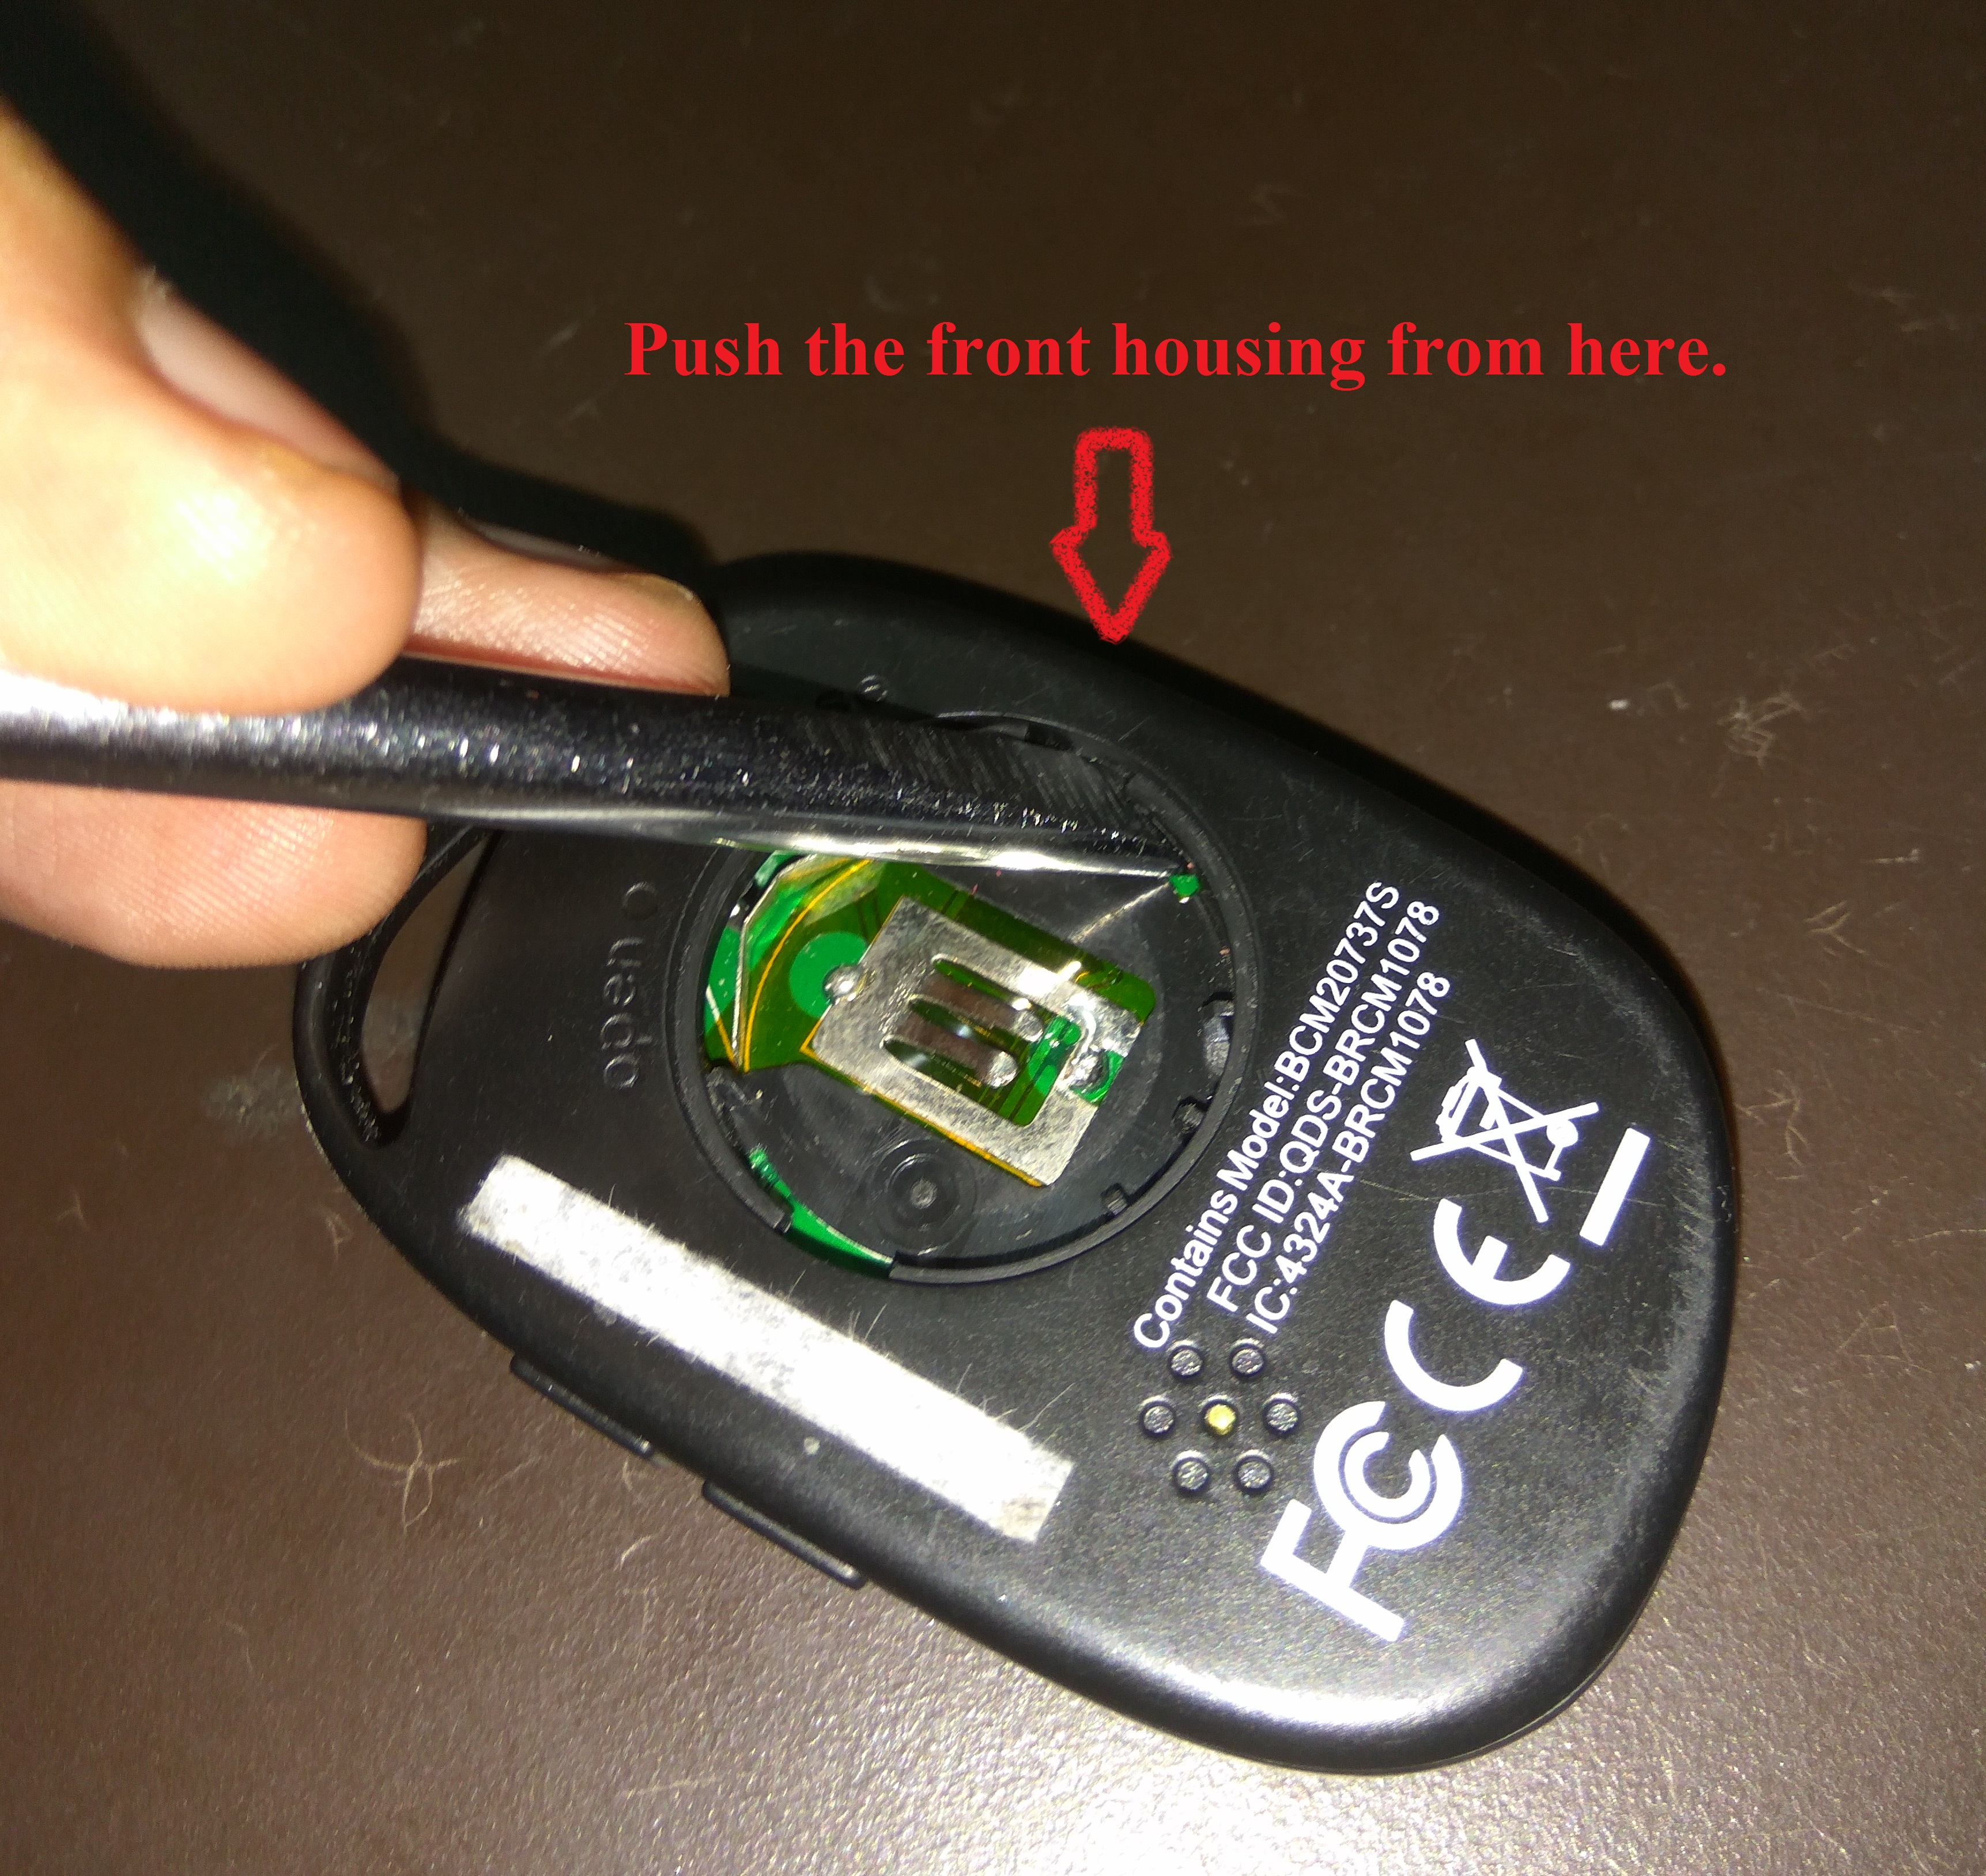
\includegraphics[scale=0.05]{3.jpg}
	    \end{figure}
	  
	  \newpage
	  \item Remove the housing in which the pcb in enclosed so as to make the boot and reset buttons visible. Remove the screws that are shown in the image.
	  
	  \begin{figure}[h]
        \centering
    	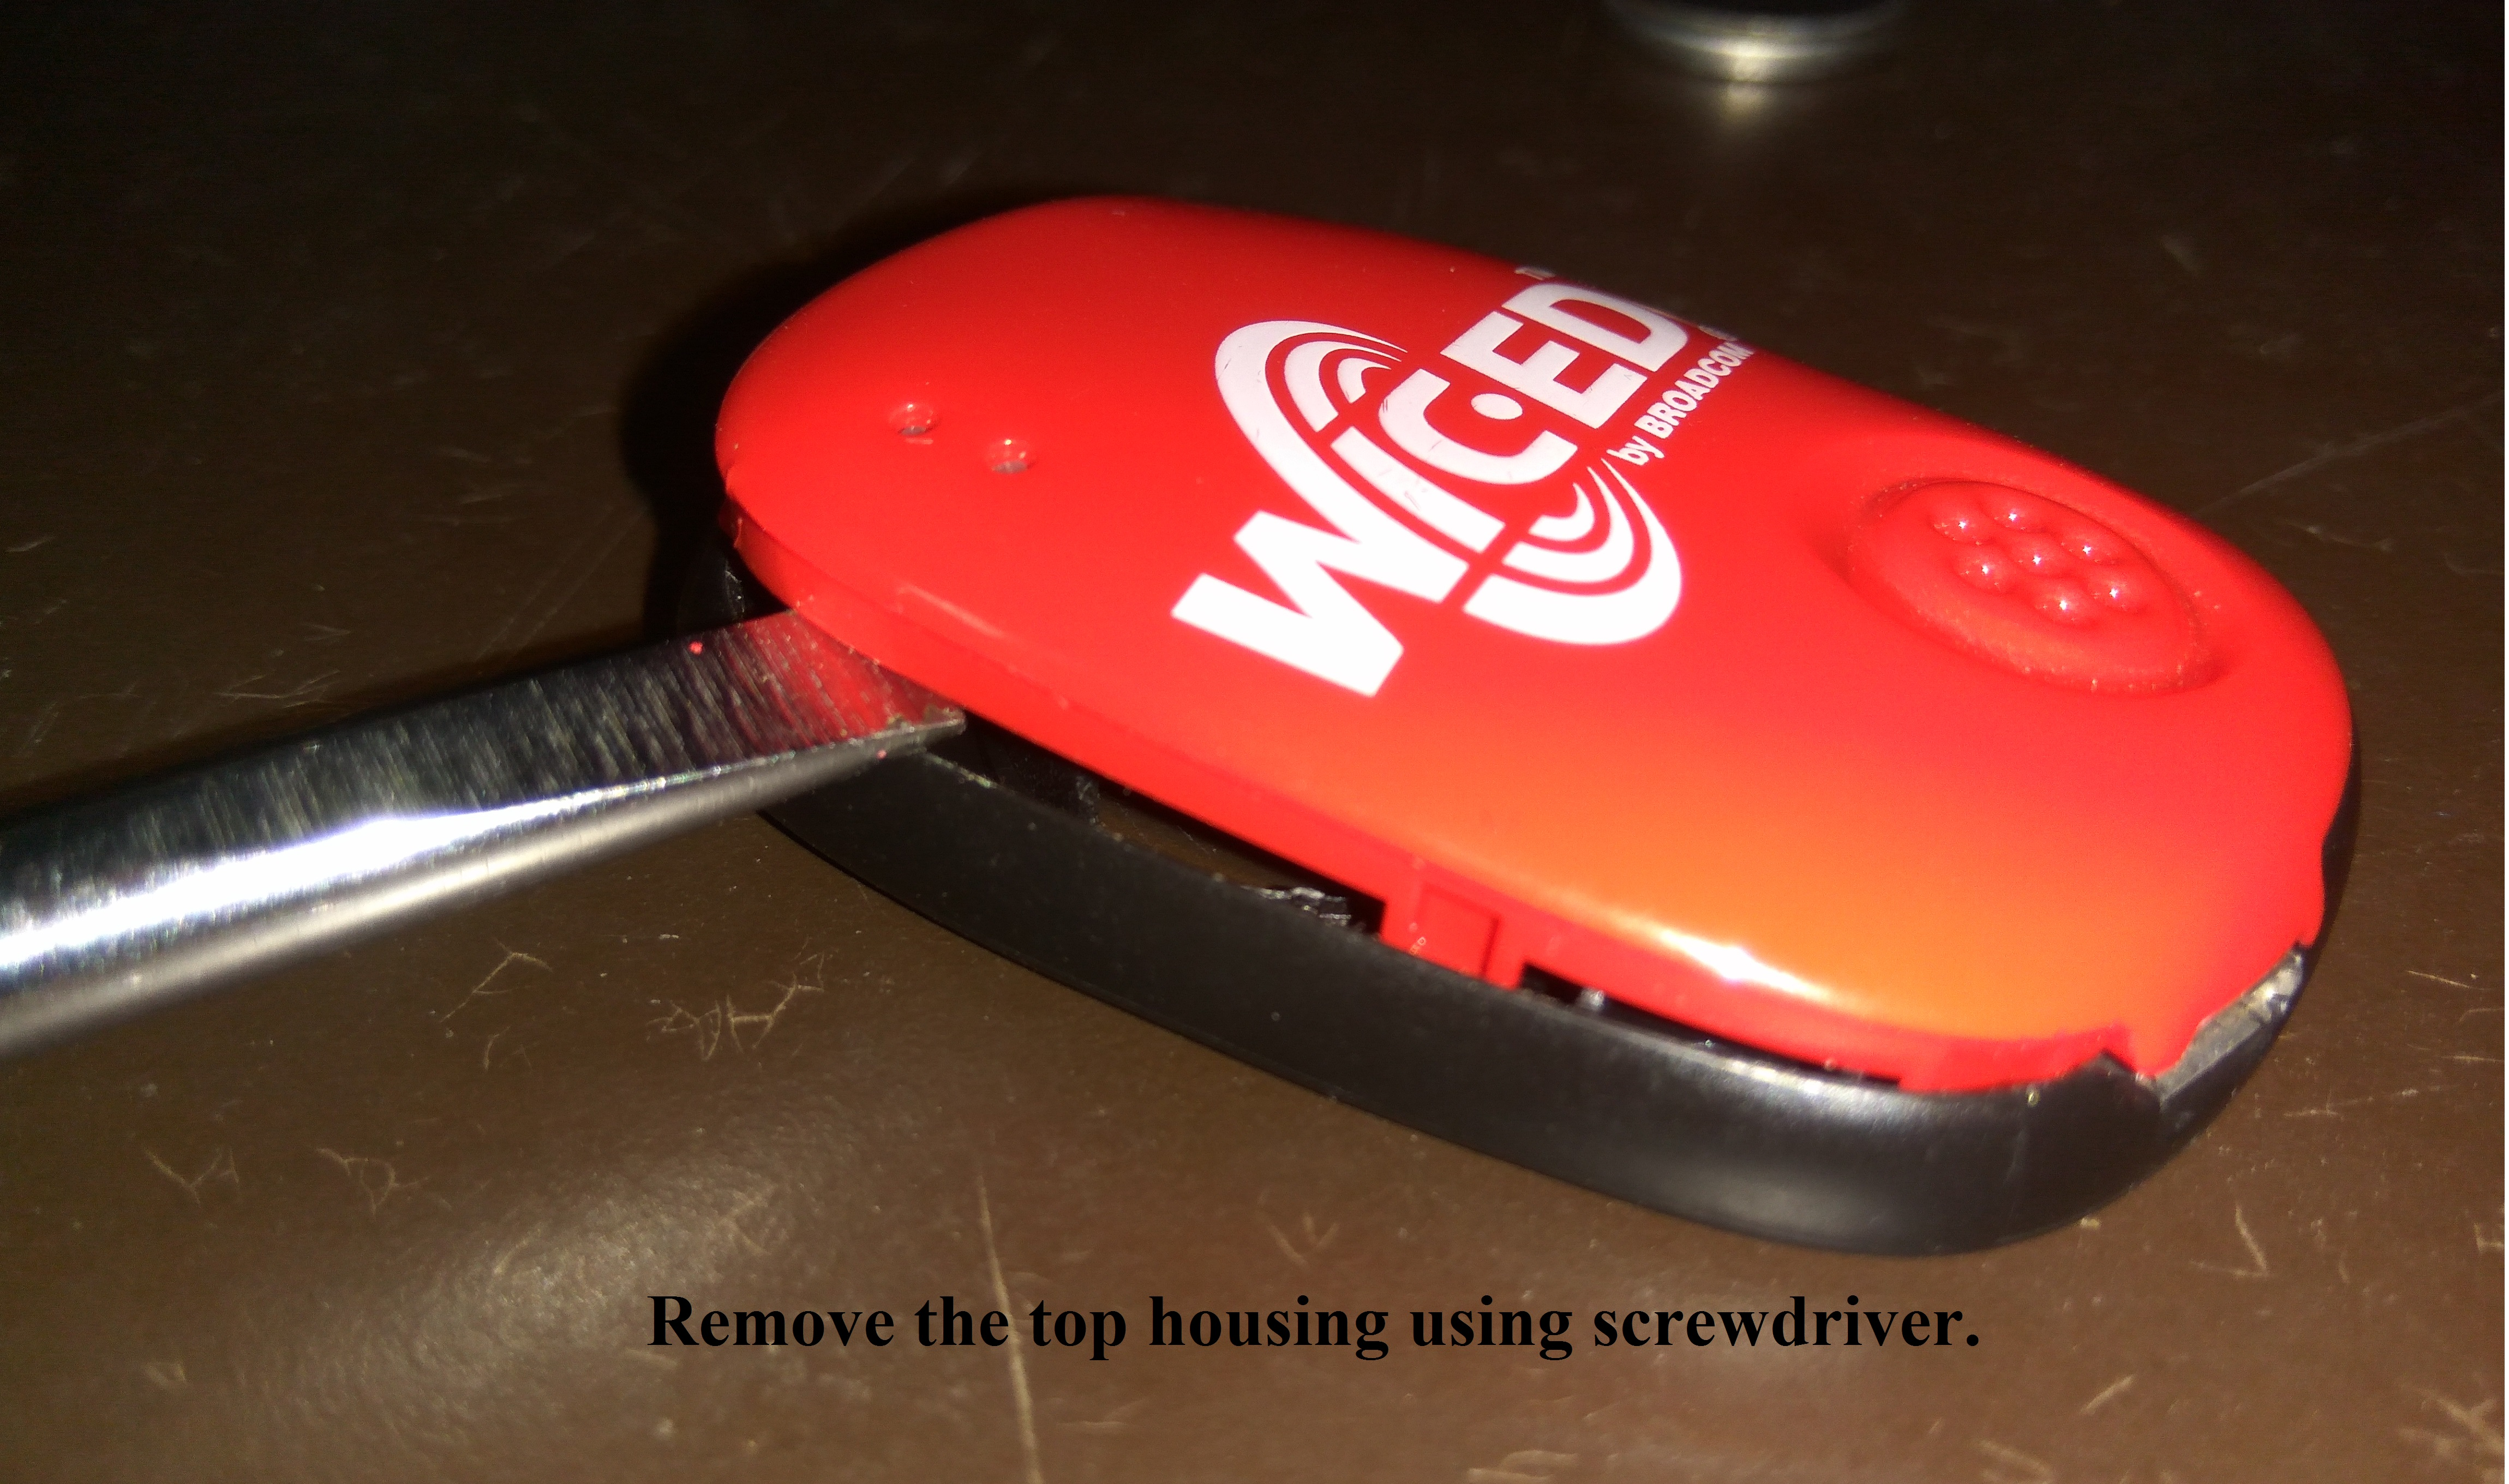
\includegraphics[scale=0.05]{4.jpg}
	    \end{figure}
	    
	    \begin{figure}[h]
        \centering
    	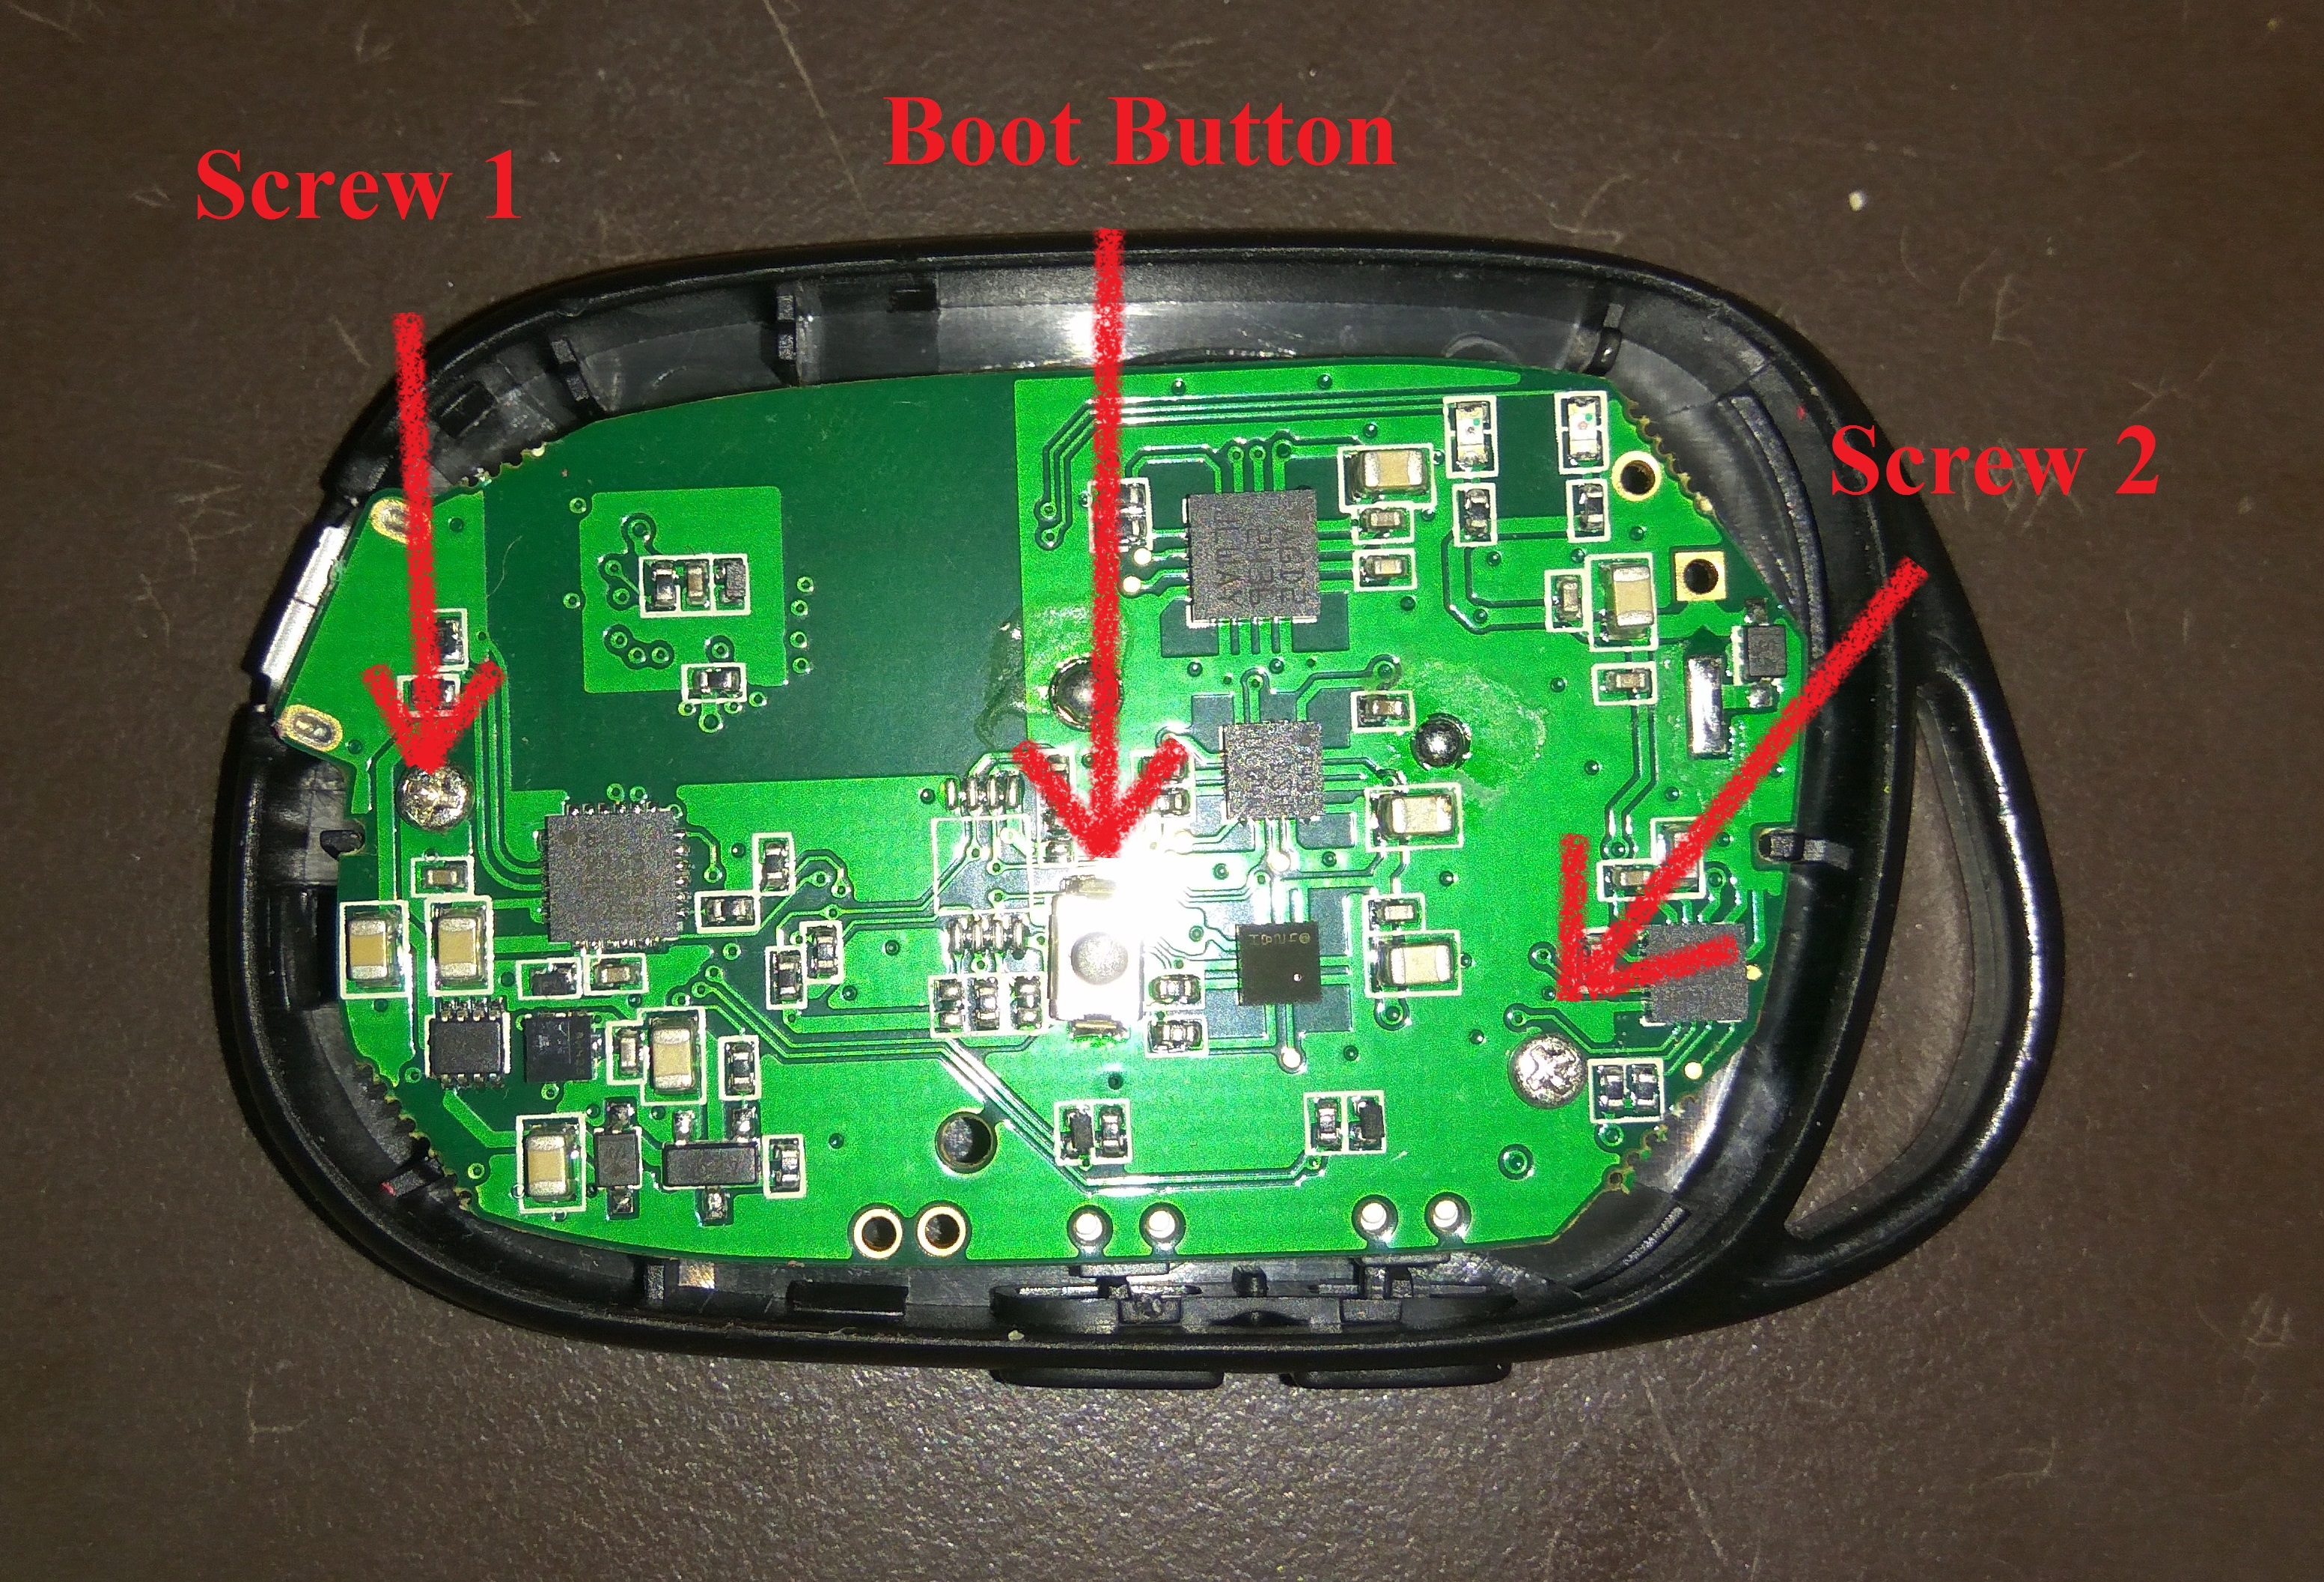
\includegraphics[scale=0.08]{5.jpg}
	    \end{figure}
	    
	    
	    \begin{figure}[h]
        \centering
    	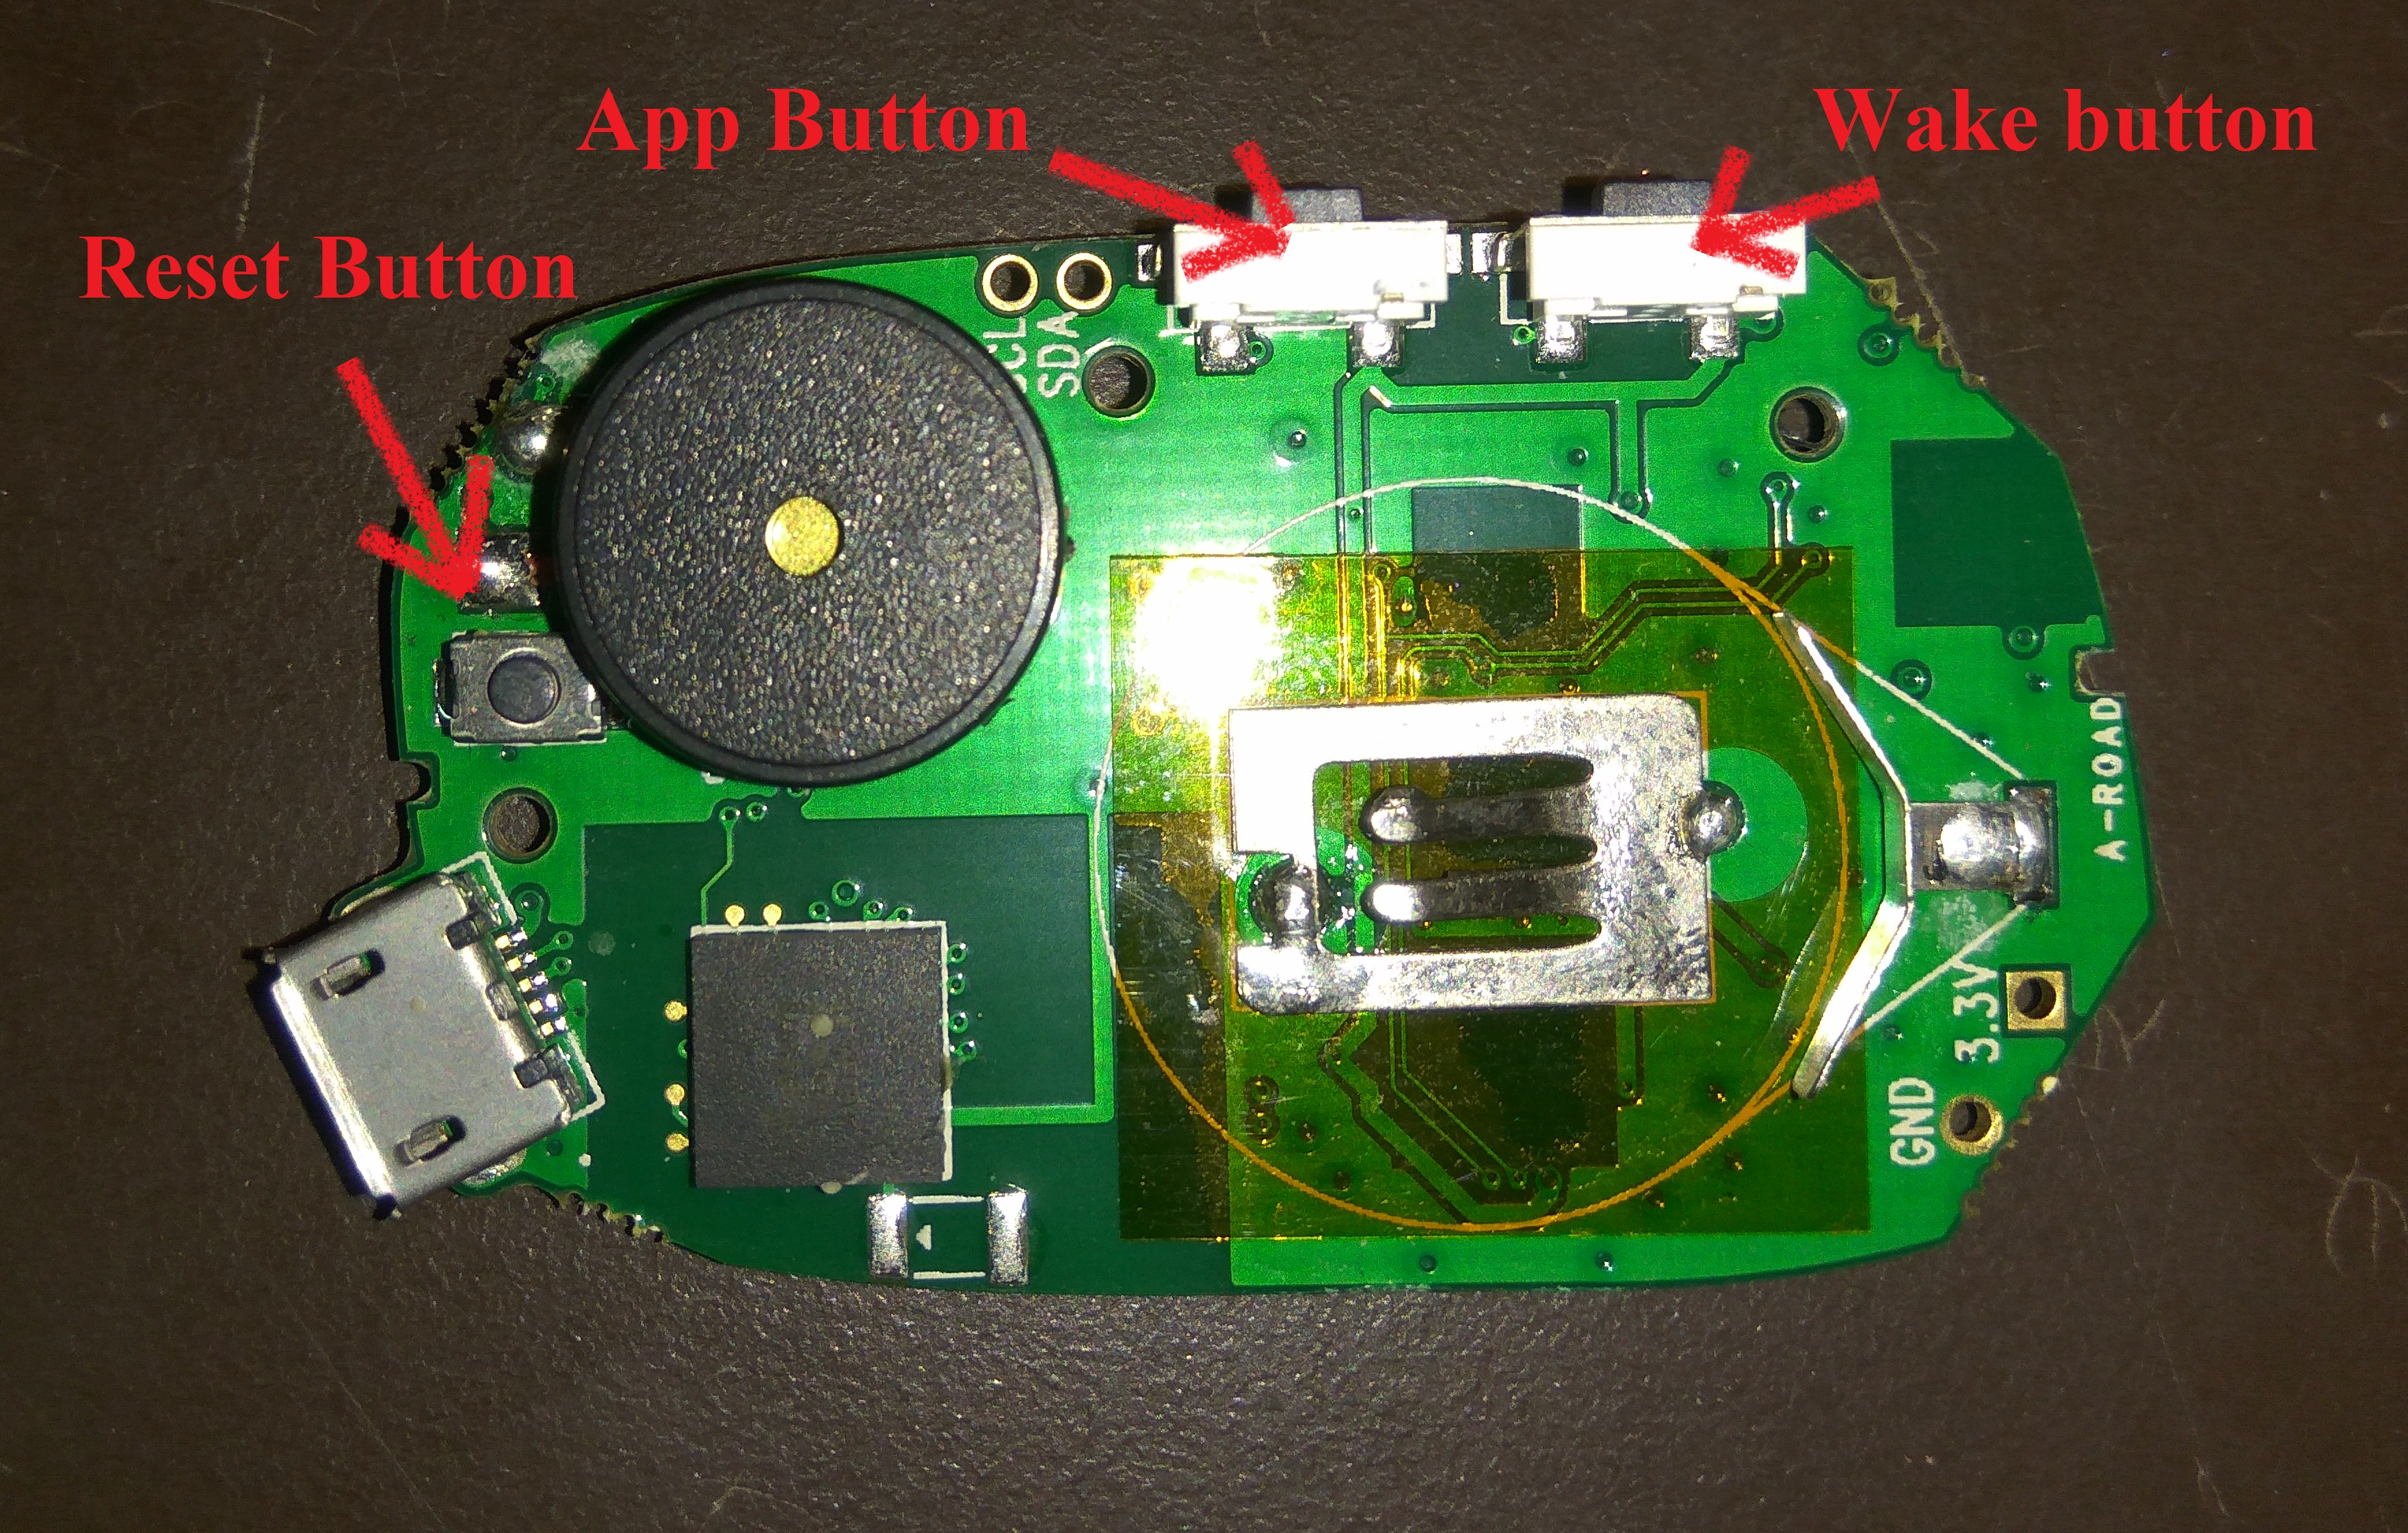
\includegraphics[scale=0.07]{6.jpg}
	    \end{figure}
	    
	  \item Follow the instructions given in Programming the Wiced Sense document for installing the Silicon Labs USB Drivers and the Wiced SDK.
	  \item Connect the USB cable to Wiced Sense Kit.
	  
	  \newpage
	  \item Go to Control Pannel > Hardware And Sound > Device Manager > Ports.
	  
	  \begin{figure}[h]
        \centering
    	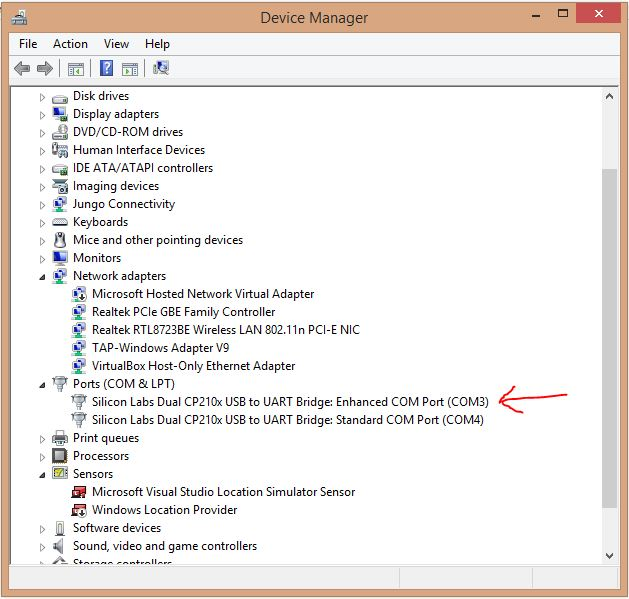
\includegraphics[scale=0.5]{comport.JPG}
	    \end{figure}
	    
	  \item Note down the Enhanced COM port on which the wiced is connected.
    \item Open the Wiced SDK.
	\item Refer the Programming Wiced with Wiced SDK document to make the target.
	
	\newpage
	 \begin{figure}[h]
        \centering
    	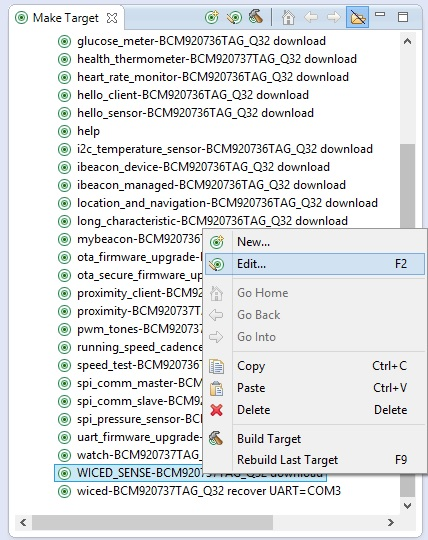
\includegraphics[scale=0.5]{edit1.jpg}
	    \end{figure}
    \item Edit the name of the target whose name was WICED-SENSE-BCM920737TAG-Q32 download to WICED-SENSE-BCM920737TAG-Q32 recover UART=COM3 in the Modify target dialog box.
    \item Note that the COM port in your system may be different. Replace COM3 with that COM port.
     \begin{figure}[h]
        \centering
    	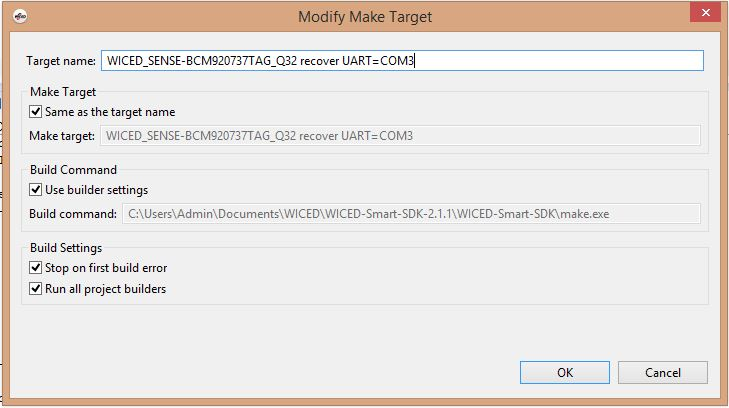
\includegraphics[scale=0.5]{edit.JPG}
	    \end{figure}
	    
	   \newpage
    \item Now all set. Double click on the target and the compiling process should begin.
    \item You can observe the output on the console.
    
    \begin{figure}[h]
        \centering
    	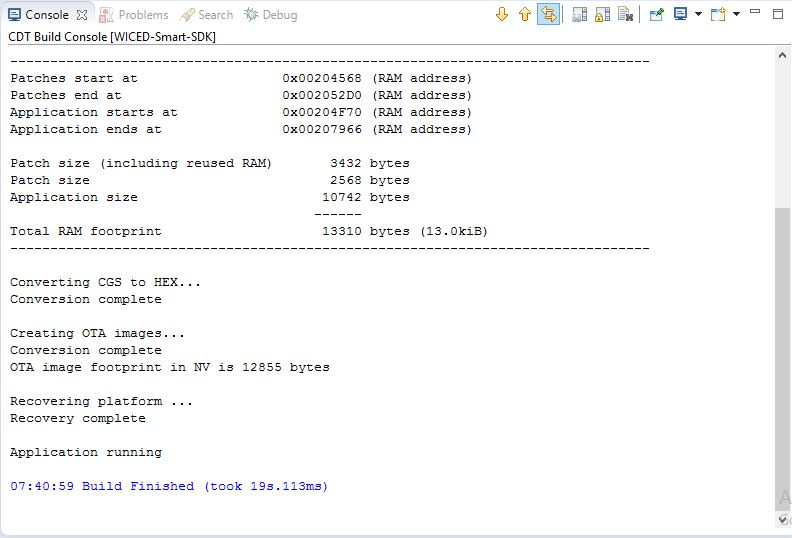
\includegraphics[scale=0.5]{recovery_complete.JPG}
	    \end{figure}
	    
    \item You will see Recovering platform and Recovery Complete on the console. At the end you will get Application Running. It means that recovering firmware was successful.

 
 	\end{enumerate}
 
 \newpage
	\section{References}
	 \begin{itemize}
	 \item https://community.cypress.com/community/wiced-smart/wiced-smart-forums/\\blog/2014/08/27/wiced-sense-ios-source-code
	 \item Refer the video in Research/Videos section.
	    \end{itemize}
 
 \end{document}